\section{Entraînement du modèle}%
\label{sec.results.training}

Tous les tests présentés dans le reste de ce chapitre ont été effectués sur un ordinateur portable 
équipé d'un processeur \verb|Intel Core i9-8950HK| et d'une carte graphique \verb|NVIDIA GeForce GTX 1050 Ti|.
Cette machine se dispose de 32 Go de mémoire vive et de 4 Go de mémoire vidéo.
Le système d'exploitation est \verb|Ubuntu 20.04 LTS|, 
la version de Python utilisée est \verb|3.10.6|
et celle de CUDA est \verb|11.6.124|.


\subsection{Choix des hyperparamètres}%
\label{sub.results.training.hyperparameters}

Pour notre premier test, nous avons entraîné le modèle pour 8 époques.
Les hyperparamètres ont été choisis comme suit :
\begin{itemize}
    \item Dimension de plongement : 64
    \item Dimension de la couche cachée : 64
    \item Taux d'apprentissage : \(3 \times 10^{-4}\)
    \item Dropout : 0.1
    \item Nombre de couches de l'encodeur/décodeur : 3
    \item Nombre de têtes d'attention : 4
    \item Norme maximale des plongements : 1
    \item Taille de lot : 256
    \item Norme maximale du gradient : 1
    \item Coefficient de régularisation \(L_2\) : \(10^{-4}\)
    \item Nombre de processus pour le chargement des données : 4
\end{itemize}


\subsection{Résultats}%
\label{sub.results.training.results}

Pour chaque époque, nous avons calculé la moyenne de la fonction de perte, de l'exactitude et du score \gls{bleu} 
sur le corpus de validation et sur le corpus d'entraînement.
Les résultats sont présentés dans la Figure~\ref{fig.results.training}.
\begin{figure}[hbt]
    \begin{subfigure}{.5\textwidth}
        \caption{Exactitude}
        \begin{center}
            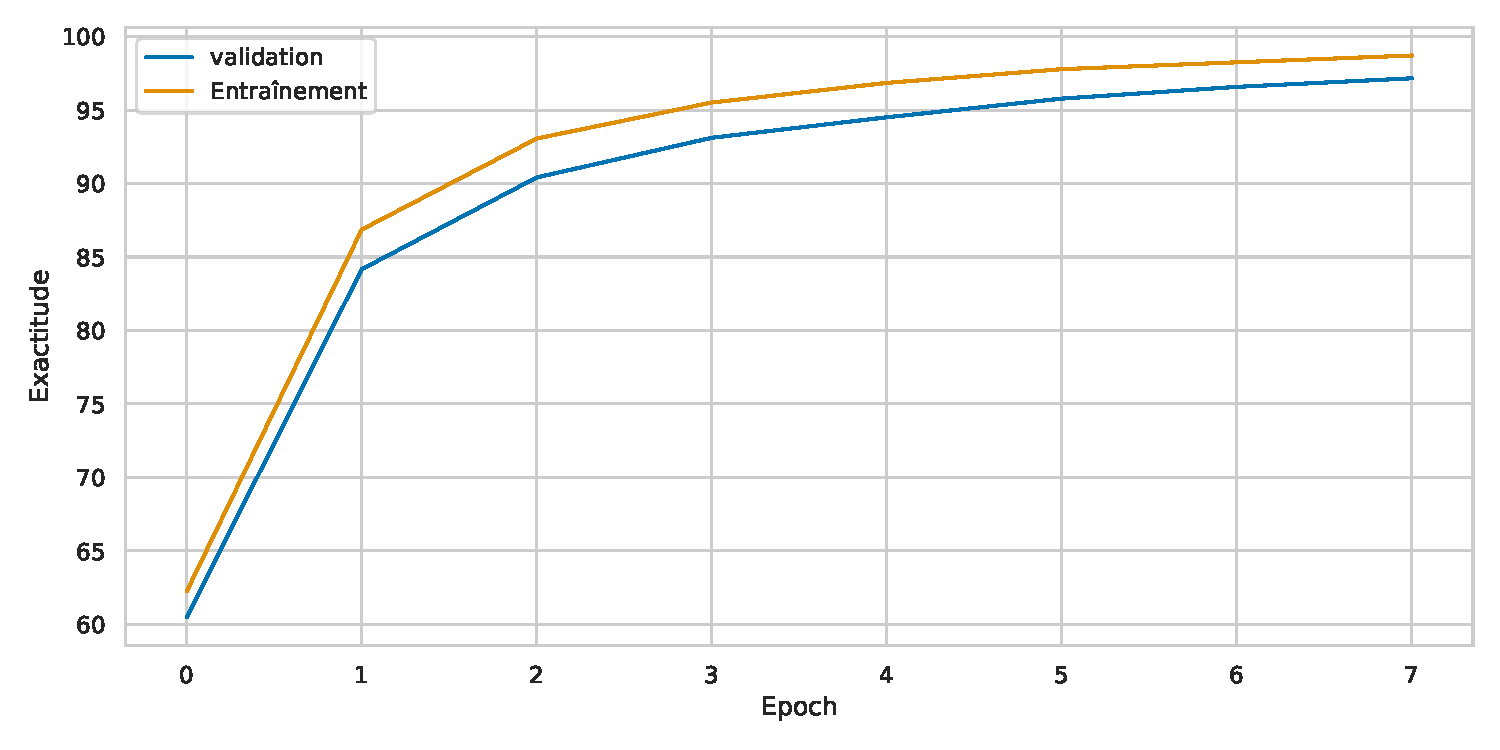
\includegraphics[width=\textwidth]{assets/python/accuracy.pdf}
        \end{center}
        \label{fig.results.training.accuracy}
    \end{subfigure}
    \begin{subfigure}{.5\textwidth}
        \caption{\glsfmtshort{bleu}}
        \begin{center}
            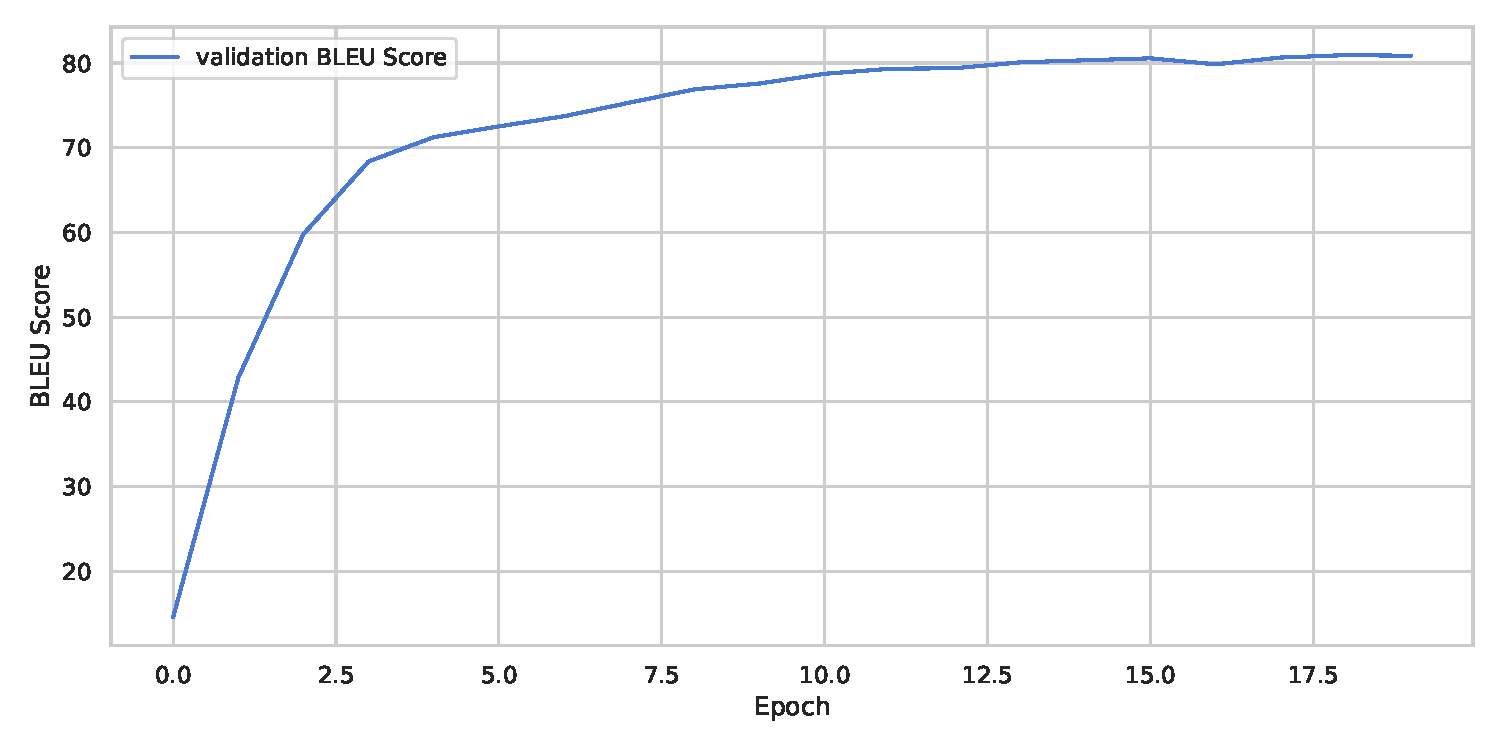
\includegraphics[width=\textwidth]{assets/python/bleu.pdf}
        \end{center}
        \label{fig.results.training.bleu}
    \end{subfigure}
    \begin{subfigure}{.5\textwidth}
        \begin{center}
            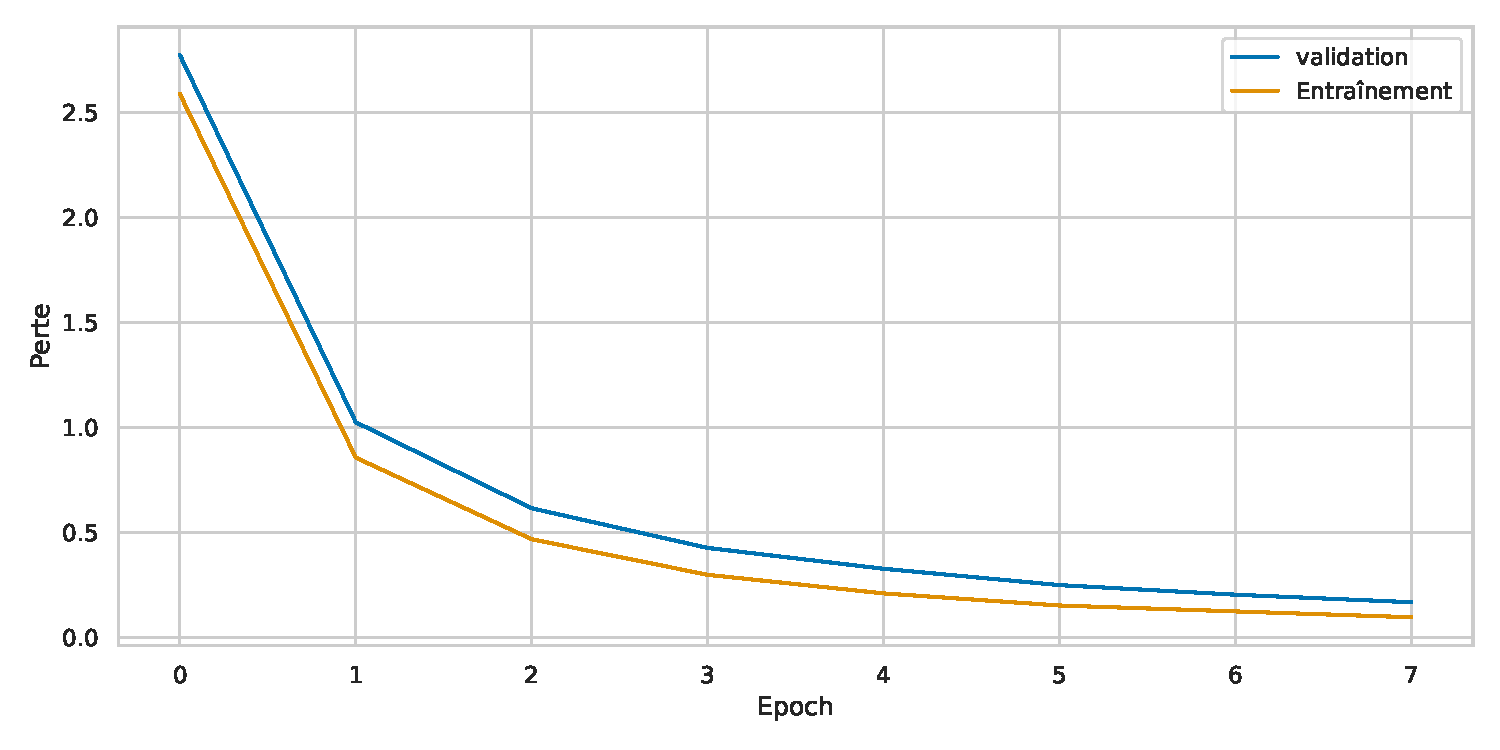
\includegraphics[width=\textwidth]{assets/python/loss.pdf}
        \end{center}
        \caption{Perte}
        \label{fig.results.training.loss}
    \end{subfigure}
    \caption{Évolution des métriques au cours de l'entraînement.}
    \label{fig.results.training}
\end{figure}
Au bout de 8 époques, la perte sur le corpus d'entraînement est de \(0.09\).
L'exactitude est de \(98.71\%\) et le score \gls{bleu} est de \(81.41\%\).
Les résultats sur le corpus de validation sont comparables.
Les mêmes métriques valent respectivement \(0.16\), \(97.16\%\) et \(77.38\%\).
Cela suggère que le modèle ne sur-apprenne pas et qu'il est capable de généraliser.
On note également que les pentes des trois courbes ne sont pas négligeables.
Il est donc probable que le modèle puisse encore s'améliorer en augmentant le nombre d'époques.